\section{Partial Tree}
\label{sec:partialtree}

The main idea of our approach for evaluating large XML documents is to 
split an XML document into chunks and query the chunks on different 
computers of a cluster. To support this, we first define the structure for presenting a chunk in
the memory, which is called a \emph{partial tree}.
The partial tree is the core concept in our research. We use partial trees
to represent chunks of an XML document and the XPath queries are also
applied to partial trees. Therefore, to begin with, we will give a
detailed introduction to the partial tree.

\subsection{Node types and definitions}

Partial trees contain many different types of XML nodes.
Four types of nodes are shown in Fig.~\ref{fig:nodetypes}.  A 
closed node has both its start tag and end tag. A node without one of 
its tags is called an open node. A left-open node is missing its start tag, 
and a right-open node is missingits end tag. 
In the figures, the missing tags are illustrated by a black
dot: $\bullet$. A pre-open node is a node missing both of its tags. 
Actually a node is no longer a node if it misses both of its tags. 
But we need it for representing the parent node of a partial tree, 
which specifies the relationships from the root. 
Note that our research focuses on querying nodes; therefore, it is not interesting 
for us that no tag is contained in a chunk, even if we can denote the whole chunk as a pre-open node. 
All the three types of nodes, left-open node, right-open node, or pre-node, are called \emph{open nodes}.
\begin{figure}[t]
	\centering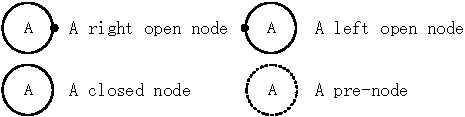
\includegraphics{partialtree/figures/fromWord-2.pdf}
	\caption{Four node types}
	\label{fig:nodetypes}
\end{figure}

\subsection{Standard Model for Partial Tree}

Now we discuss the characteristics that partial trees generally
have. Since the left-open nodes, right-open nodes, and pre-nodes are the special nodes in
partial trees, we focus on the properties of the open node.

The first property is about the parent-child relationship of the open
nodes.

\begin{property}
\label{property1}\itshape
If a node on a partial tree is left/right open, then its parent is also left/right open.
\end{property}

The second property is about the sibling relationship of the open nodes. 

\begin{property}
\label{property2}\itshape
If a node is left open, it is the first node among its
siblings in the partial tree. If a node is right open, it is the last
node among its siblings in the partial tree.
\end{property}

There is another important property of pre-nodes.

\begin{property}
\label{property3}\itshape
If there exist multiple pre-nodes, then only one of
them has left-open/closed/right-open nodes as its child.
\end{property}

We develop a standard model of partial trees  based on these properties
as shown in Fig.~\ref{fig:model}.

\begin{figure}[t]
\centering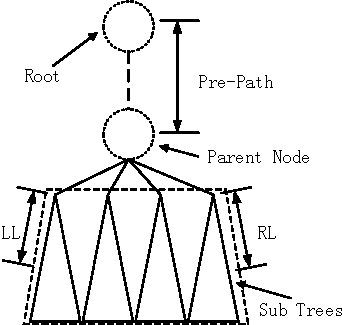
\includegraphics{partialtree/figures/fromWord-4.pdf}
\caption{A standard model of partial tree.}
\label{fig:model}
\end{figure}
 
The partial tree consists vertically of two parts: a list of pre-open
nodes and a forest of subtrees. We call the list of pre-open nodes
\emph{pre-path}. The pre-path plays an important role in applying queries from the root. 
From property~\ref{property3}, one or more subtrees connect to a pre-node at the bottom of
the pre-path. Note that for each subtree, there is only one root, which is
a left-open/closed/right-open node, but there could be one or more subtrees. 

From properties \ref{property1} and \ref{property2}, 
we know that the left-open nodes are located on
the upper-left part of a partial tree and the right-open nodes are located on the
upper-right part. More precisely, the left-open nodes form a list from a
root node of a subtree, and we call the list the \emph{left list} (LL). Likewise, we call the
list of right-open nodes the \emph{right list} (RL). 